\documentclass[12pt]{scrartcl}

\usepackage{fullpage}
\usepackage{graphicx}
\usepackage{setspace}
\doublespacing

\title{Honors Thesis}
\author{Gina Chun}


\begin{document}

\maketitle

\newpage

\begin{abstract}
  Abstract...
\end{abstract}

\newpage

\tableofcontents

\newpage

\section{Introduction}\label{Introduction}

\subsection{Why Carbon is Important}

% In this section to say blah

Carbon is one of the most important and widely investigated
elements. Carbon is all around us in a variety of forms and is an area
of study which has huge significance across many scientific fields and
applications. Carbon is in living organisms and is essential for
living organisms, thus the study of carbon would further develop the
complex workings of the environment, ecosystems and the carbon
cycle. It would also help the understanding of fossil fuels, aid the
challenges of energy-related issues, and work towards solutions for
climate change. Carbon materials are also intertwined in modern
economic industries such as in steel, clothing, pigment, plastic and
synthetic materials, and in electrodes and other similar electricity
conducting machinery. Studying carbon allows for further advancement
in these important industries which would lead to better and more
easily accessible devices, tools, and products for general society.

\subsection{Why Use Machine Learning}
As carbon is an important element, its versatility makes it a very
complex subject of study. Carbon manifests in various physical forms,
called allotropes, each with very different properties. Because of
this, studying carbon can be difficult with conventional
methods. Using Gaussian Approximation Potentials (GAP), machine
learning can be much more cost and time efficient than traditional
scientific methods of experimentation. Machine learning also opens up
a new space of empirical methods for experiments that scientists
cannot physically replicate with traditional techniques. For example,
machine learning can be used for experiments in very small spatial
scales or for large scale simulations all while maintaining high
performance accuracy.

\newpage

\section{Background}

\subsection{Chemistry}

% Machine Learning Meets Quantum Physics textbook
% Introduction to material modeling
Using machine learning to study any kind of material, not just carbon, 
is just one method under a wider category of techniques called material modeling. 
Material modeling in chemistry is the method of using computer simulations to predict 
physical and chemical properties of a material in replace of real-world experiments. 
This process of predicting the properties of a given material is called a \emph{forward 
problem}. Through existing tools such as statistical mechanics and the Schrödinger 
equation, which will be talked about later, an exact unique solution exists for the 
forward problem of predicting material properties and is the reason why many opt to 
use this procedure. Material modeling also uses this approach because the inverse 
problem, constructing a material through a set of pre-determined properties, 
is much more difficult and costly to do.

\subsubsection{Geometry and Structure}
% Structure property relation for molecules
``Structure determines properties'' is a very important and central concept in chemistry. 
This structure-property relationship explains that since all materials are made of atoms, identifying 
and describing a material comes down to simply understanding its atomic structure. For studying 
structures, there is never a need to look at the entire material as well. That would be too many 
atoms to study at once and atoms of most solid materials, like crystalline carbon, are arranged in 
an organized repetitive pattern so it is sufficient enough to look at just a patch of that pattern. 
Studying the properties of a microscopic structure, in general, translates well to its macroscopic 
structure which allows it to pair well with the material modeling approach.

\begin{figure}
  \centering
  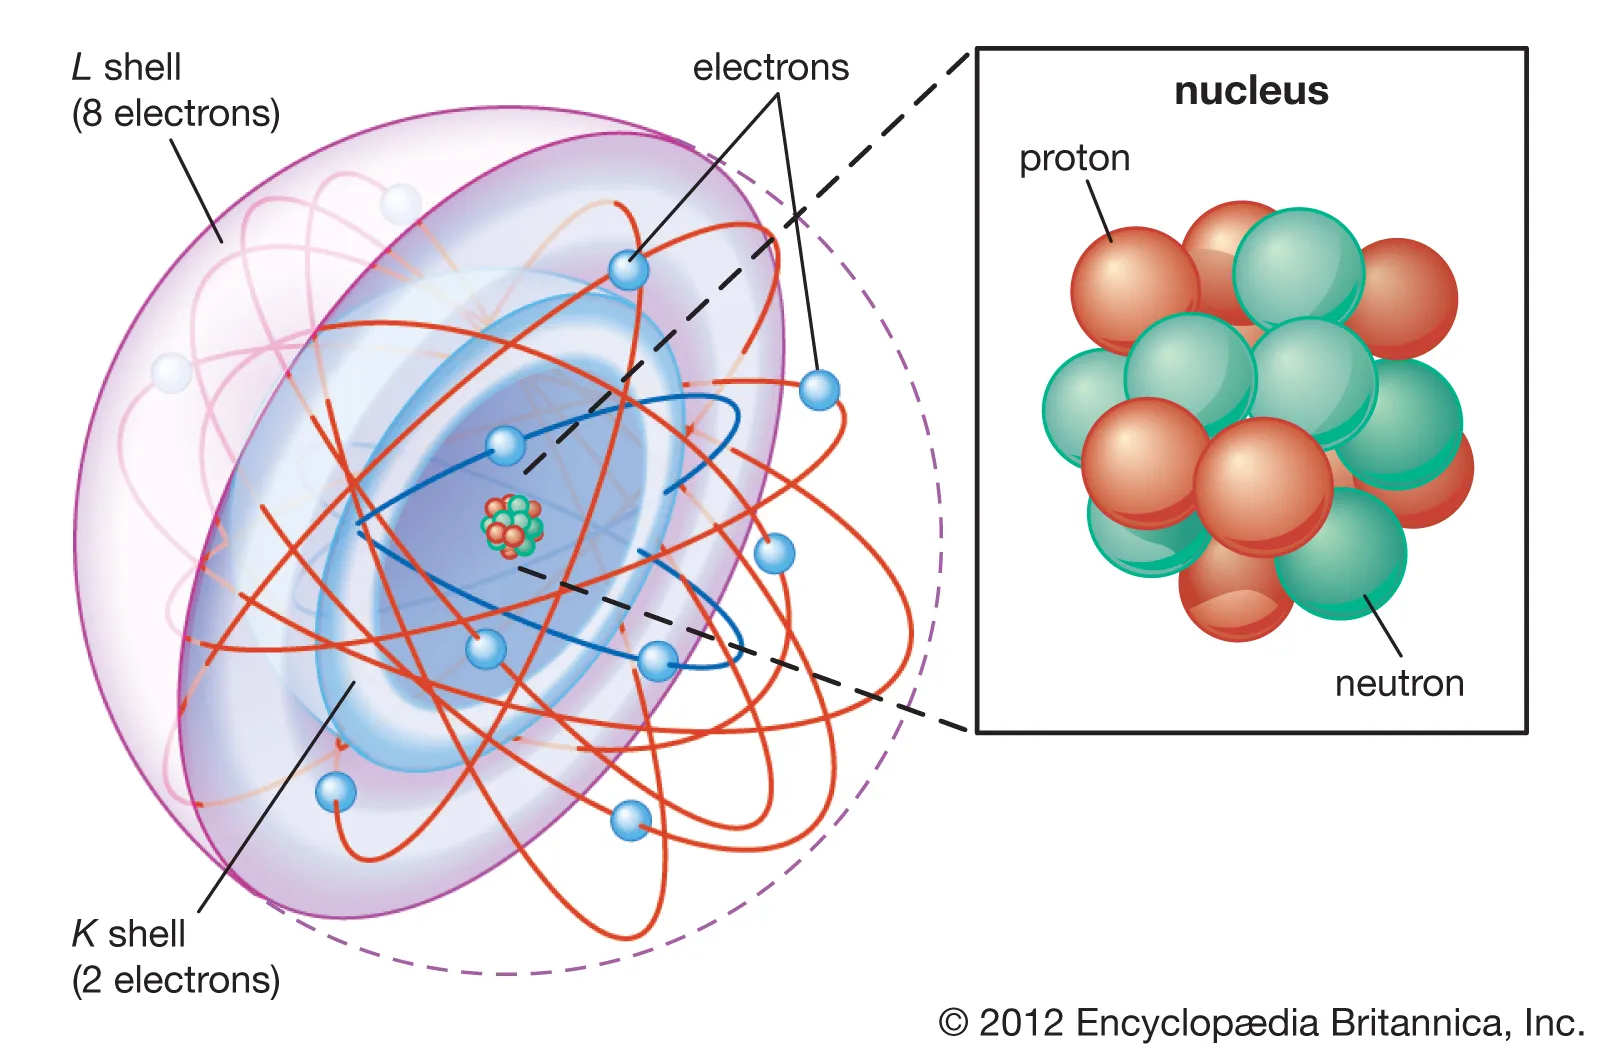
\includegraphics[scale=.25]{atom.png}
  
  \caption{Model of an atom}\label{fig:atom}
\end{figure}

% molecular \& material properties: Electronic properties (for hard degrees of freedom, crystalline)
% Born–Oppenheimer approximation, ground state, atomization energy
An atom can be described as having a heavy nucleus surrounded by a cloud of light 
electrons and since the mass of an atom is concentrated on its nucleus, the atom's 
position is associated with the position of the nucleus. Thus moving atoms can be described
as moving nuclei being followed by their clouds of electrons, as shown in figure \ref{fig:atom}. 



The Born–Oppenheimer approximation is the mathematical formulation of this concept and 
is the foundation of material modeling. Molecular and material properties can be 
roughly divided into two categories: electronic and thermodynamic properties. Electronic 
properties are essentially the properties of that electron cloud that is following the 
nucleus and is best described through quantum mechanics, which will be covered in more 
detail later. To give a general overview, the electronic cloud can be in certain states 
such as its lowest-energy state called the \emph{ground state}. Some ground state properties include the atomization energy, which is the energy released when a molecule is formed, and the 
dipole moment and polarizability, which describes the shape and responsiveness of the
cloud. Since thermodynamic properties can be more easily derived through knowing the electronic 
properties first, this paper and its method will be predicting ground-state electronic properties 
so that is what the background will be focused on. 


\subsubsection{Quantum Mechanics}
% object being in multiple states
% Schrödinger equation, DFT, PES
% computational cost with solving the equation
Quantum mechanics is the set of laws that describe objects on an atomic level. One of the core
principles is that an object can be in multiple states. An object like an electron can be in any 
combination of these two states. Mathematically, this can be expressed as a linear combination of 
two basis vectors that act as the two position states. The state of this object can be expressed 
as a \emph{wave function}, which generalizes the two position vectors to the infinite number of 
positions in the three-dimensional space. This fundamental idea is why electrons are commonly 
referred to as clouds.

The laws of quantum mechanics also states that each observable, quantifiable, physical property that 
an atomic object has is associated with a linear operator. The actual value of the quantity is given 
by the eignevalues of the operator. One of the most important operators is the energy operator, called 
the Hamiltonian, and its associated eigenvalue equation is called a Schrödinger equation. The energy of 
a particular eigenstate as a function of the nuclear positions is called a \emph{potential energy surface}
and it completely determines the dynamics of the motion of the atoms. The solution to this equation 
allows many electronic properties of both ground and excited states to be determined. The Schrödinger 
equation can be mathematically solved for singular atoms but it gets more difficult for more complex molecules. 
There are methods such as the density functional theory and the Hartree-Fock that try to 
solve this issue by manipulating the Hamiltonian or the vector space itself, but their computational 
costs make these methods practically inefficient. Once the Schrödinger equation is solved, evaluating 
properties such as atomization energy or dipole moment can be done through the eigenvalues and eigenstates.

\subsubsection{QM Software} 
Currently, there are programs used in computational chemistry to implement the methods mentioned above to 
calculate properties.One software, called Vienna Ab initio Simulation Package or VASP, performs ab initio 
quantum mechnical calculations and uses DFT as its base methodology. Another software package, called 
QUantum Mechanics and Interatomic Potentials or QUIP\cite{quip}, has a collection of tools to conduct 
molecular dynamics simulations and works with other external packages such as LAMMPS or ASE. This paper 
will use the QUIP software as reference calculations to experimental results. The Carbon GAP 20 
potential\cite{gap20} will be used as the parameters in the QUIP calculations.

\newpage


\subsection{Machine Learning}

% graph representation (molecules as graphs)
% types of problems that use graph structured data 
In a molecule, different pairs of atoms and bonds have different distances so it is easy to describe
these molecules as a graph. The atoms are the nodes and the bonds are the undirected edges. In general, 
there are three types of prediction tasks that are done on graphs: graph-level, node-level, and edge-level. 
Graph-level approaches predict a single property for a whole graph while a node-level approach predicts 
a property for each node in the graph. Edge-level approaches predict the property or existence of edges 
in a particular graph. This paper focuses on the graph-level task of predicting the energy of carbon 
molecules. 

% integrating graphs in neural networks (matrices, adjacency lists)
Integrating these graphs into machine learning models will depend on how they are represented. 
An obvious representation method would be the adjacency matrix since it captures the graph's connectivity. 
However, the more nodes there are, the more space-inefficient the adjacency matrix becomes and in addition,
the adjacency matrix of a molecule is not unique. There are many different ways to express the same 
connectivity with these matrices which causes the model to be permutation invariant since it will see 
these matrices as different molecules when they are actually the same. A better memory-efficient representation 
is adjacency lists where each item in this list describes the connection between just two nodes. This cuts out 
a lot of the parts of the graph that are disconnected that would be needlessly recorded in an adjacency matrix.


\subsubsection{Graph Neural Networks}    

% Pooling and Message Passing
A graph neural network (GNN) consists of transformations on all attributes of the given graph 
that preserves its symmetries and thus is permutation invariant. The simplest kind of GNN has 
each layer apply a multilayer perceptron (MLP) on each attribute of a graph which includes the
nodes, edges, and global-context. Since predictions are made on the nodes of the graph, \emph{pooling} 
is a way to gather information about the edges and give them to the nodes. This is done by 
gathering the embeddings of each item that will be pooled into a matrix and then aggregate them, 
usually through a summation. More complex predictions can be made by using pooling 
in each of the GNN layers which lets information exchange influence updated embeddings. This 
allows the embeddings to be aware of the graph's connectivity and is called \emph{message passing}. 
The forward pass of a message passing neural network (MPNN) consists of two steps: message passing 
and readout. In message passing, each node has a hidden state or feature vector and a function of 
neighboring hidden states are aggregated for each node. The hidden state of a node is updated using 
the obtained message and the previous hidden state of that node. Conceptually this allows each node 
to understand and use previous history to influence their future update. The readout step computes 
a feature vector for the whole graph.

% Graph convolution
\begin{figure}
  \centering
  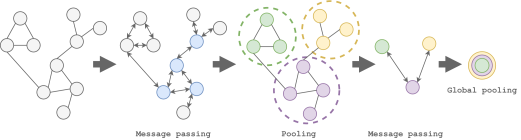
\includegraphics[scale=.75]{mpnn.png}
  
  \caption{Simple example of message passing in a graph}\label{fig:mpnn}
\end{figure}

A specific way to carry out message passing is by using graph convolutions. Just like in convolutional 
neural networks, the input is multiplied by a set of weights known as \emph{kernels}. It acts like a 
filter that scans across the input graph and allows the model to learn features from neighboring nodes, as shown in figure \ref{fig:mpnn}.
Convolutions collect and condense information about local environments within a graph to learn about 
its connectivity. Through this kernel, neighboring information can be aggregated with the information 
the node is already holding and thus performs message passing throughout the convolutions.




\newpage 

\section{Method}
\subsubsection{Training Dataset}\label{Train}
%Carbon GAP 20 data
The training data is from a dataset called Carbon GAP-20 Training Set\cite{gap20}. It contains 6,088 configurations of mostly crystalline carbon and some liquid and amorphous carbon with their respective atomization energies. As shown in figure \ref{fig:train}, the dataset is very comprehensive for all possible crystalline phases of carbon at moderate temperatures and pressures with the additional inclusion of more exotic allotropes. It also has DFT optimized structures for graphite, graphene, cubic and hexagonal diamond. 

% Graph dataset
This dataset of geometries is then turned into a graph dataset. For each atom in each molecule, four nearest neighbors are found and the distances are calculated to that atom. Once the the distances for the four nearest neighbors of each atom is found, it is used to create a DGL\cite{dgl} graph that represents the whole molecule where the edge features of the graph contain the distance information. This method of representation uses the local environment of each atom to describe a whole molecule and determine its energy. This representation is both rotation and translation invariant. This is because the distance between these atoms do not change if rotated or translated, thus it does not depend on its specific Cartesian location.

\begin{figure}
  \centering
  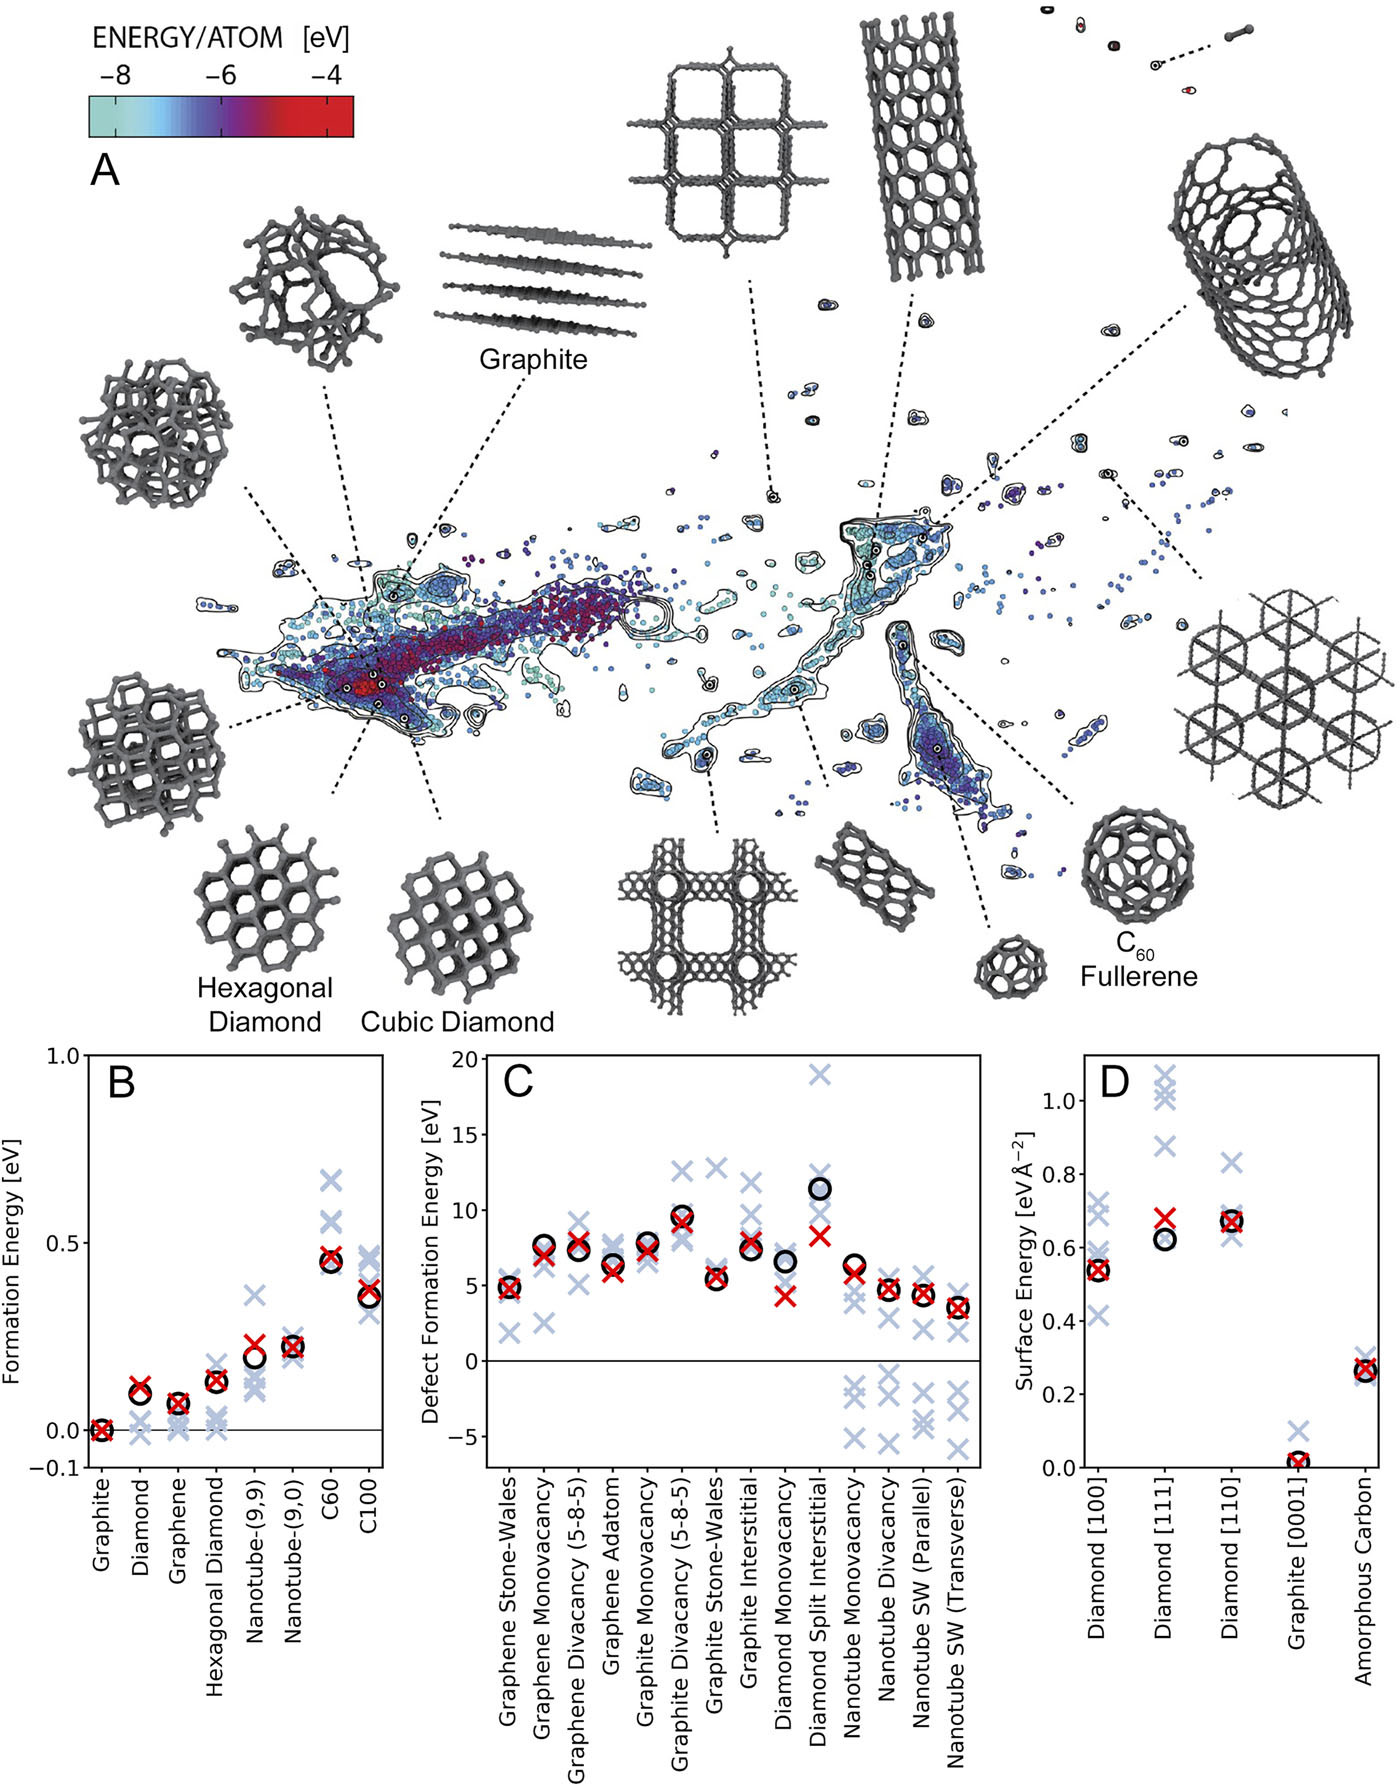
\includegraphics[scale=2]{carbon}
  
  \caption{Map of the training data with some of the key structures (top). Summary of predicted formation energies, defect formation energies, and surface energies of crystalline carbon (bottom)}\label{fig:train}
\end{figure}

\newpage
\subsubsection{Model} 
% Model
The model uses the python package DGL-LifeSci\cite{dgllife} which allows an easy integration of tasks in 
chemistry and graph neural networks. The implemented model is split into three parts: message passing, 
readout, and linear layers. The message passing graph neural network (MPNNGNN) from DGL-LifeSci first starts 
with a linear and ReLU layer. Then there is a cycle that consists of a graph convolution layer, another 
ReLU layer, and a multi-layer gated recurrent unit (GRU). This cycle is repeated for the number of 
messsage passing set in the beginning and through this repetition, node representations are being updated 
and message passing is being performed. The second part of the model is a MLP-based readout where it 
updates node representations with a MLP and then computes graph representations out of those node features. 
The third part of the model is a simple combination of linear, dropout, ReLU, linear layers.

% Permutation Invariance
An important property of this model is that it is permutation invariant. This means that the output of 
the network does not depend on the order of the input. To put it another way, say that there is a singular
water molecule with its atoms labeled "oxygen", "hydrogen 1", and "hydrogen 2". The two hydrogen atoms 
are not conceptually different in this molecule so it should not matter if "hydrogen 2" gets inputted 
before "hydrogen 1" in the model. This model is permutation invariant because nodes are communicating 
between each other and are learning from local graph information through message passing. Message passing 
allows the nodes not to be dependent on a particular input and its order.

\subsubsection{Test Dataset} 
% DUNN and Modified Total
Two datasets are used to test the performance of the model. One dataset contains carbon allotropes of monolayer graphene, bilayer graphene, graphite, and diamond with their DFT energies calculated using VASP. For simplicity, this dataset will be called the DUNN dataset for it was originally used to develop a Dropout Uncertainty Neural Network potential\cite{dunn}. The second test set comes from the source of the training set. That paper\cite{gap20} provides two datasets where the training set is a subset of the total dataset of carbon configurations. The training data was removed from the total dataset to create a Modified Total dataset to test on. The graph dataset versions of these test sets are created the same way the training graph dataset was made, referenced in section \ref{Train}. 

% Dummy, Untrained, and QUIP
Three other measurements were made to additionally evaluate the model performance. The first measurement uses the dummy regressor from Scikit-learn to make predictions and calculate its mean squared error (MSE) on both the DUNN and Modified Total test set. The second measurement uses the untrained version of the model to directly calculate predictions and MSE for both test sets to see how the model performs without any learning. The third measurement uses the QUIP software and the GAP 20 potential\cite{gap20} to calculate energies and MSE on both test sets once again. This measurement will allow the direct comparison of the cited research's results with this paper's results.


\newpage

\section{Experimental Evaluation}
\subsubsection{Results} 
Experiments were started with 1 and 3 rounds of message passing with a batch size of 16, learning rate of 0.001, and 4 nearest neighbors. Those runs were not training the model as well as it could have because they had very unstable train and test losses. The next stage of runs increased the number of message passing to 5 but those as well had unstable test losses even when the train losses were stable. 

% graph of unstable runs?

Because of this, the next round of runs kept the number of message passing at 5 but lowered the learning rate and varied the batch size. 

First, the results clearly show that the model is training. All the experiments produce an MSE lower than the untrained model for both test sets which shows that the model is working. Almost all the runs also have an MSE lower than the dummy regressor baseline which proves it is learning better than a predictor with a simple strategy. The runs compared to themselves also show that the model is definitely getting better as the parameters are adjusted because the MSE is lowering at several magnitudes between each other.

% graph
\begin{figure}
  \centering
  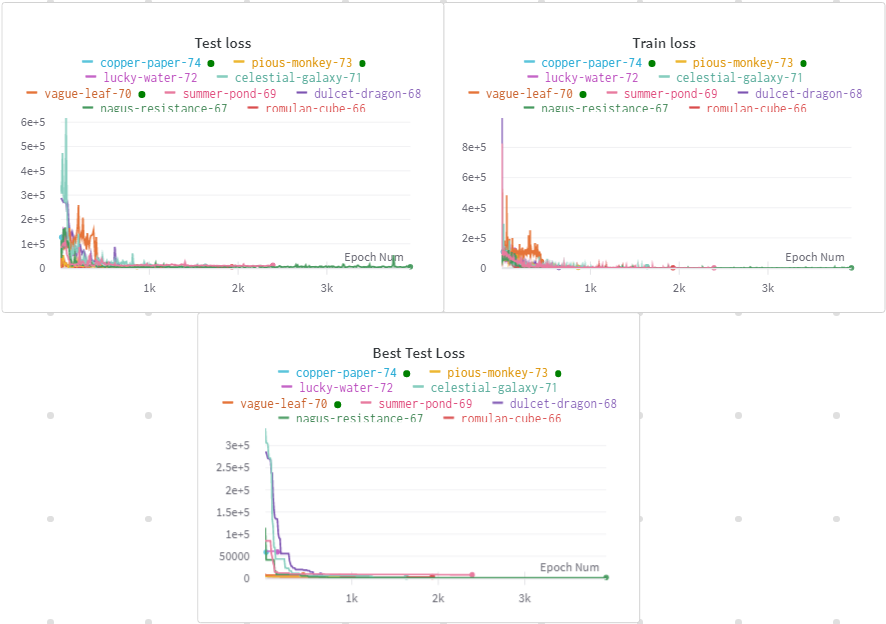
\includegraphics[scale=.75]{graph.png}
  
  \caption{wandb, place holder}\label{fig:graph}
\end{figure}

\begin{center}
    \begin{tabular}{|p{2cm}||p{2.5cm}|p{2cm}|p{2cm}|p{2cm}|p{2cm}|}
    \hline
    \multicolumn{6}{|c|}{DUNN Dataset} \\
    \hline
    Run  & MSE (ev) & Message Passing & Learning Rate & Batch Size & Nearest Neighbor\\
    \hline
    QUIP   & 45.256 &   &  &  &\\
    1   & 1,655.831 & 0.0005 & 5 & 16 & 4\\
    2 & 18,836.808 & 0.0001 & 5 & 32 & 4\\
    Dummy & 25,620.847 &   &  &  & \\
    3    & 43,933.238 & 0.0005 & 7 & 32 & 4\\
    Untrained & 228,335.155 & 0.0005 & 5 & & 4\\
    \hline
    \end{tabular}
\end{center}

\begin{center}
    \begin{tabular}{|p{2cm}||p{2.5cm}|p{2cm}|p{2cm}|p{2cm}|p{2cm}|}
    \hline
    \multicolumn{6}{|c|}{Modified Total Dataset} \\
    \hline
    Run  & MSE (ev) & Message Passing & Learning Rate & Batch Size & Nearest Neighbor\\
    \hline
    QUIP   & 16.989 &   &  &  &\\
    1   & 3,388.47 & 0.0005 & 5 & 16 & 4\\
    2 & 7,583.152 & 0.0005 & 7 & 32 & 4\\
    3    & 8,438.149 & 0.0001 & 5 & 32 & 4\\
    Dummy & 191,405.849 &   &  &  & \\
    Untrained & 418,529.850 & 0.0005 & 5 & & 4\\
    \hline
    \end{tabular}
\end{center}



\subsubsection{Suggestions} 
working on the hyperparameters more

exploring hypergraphs where you use ternary edges to represent angles
\newpage

\section{Conclusion}

\newpage

\bibliographystyle{plain}
\bibliography{ref}


\end{document}
